\documentclass[12pt]{article}

\usepackage{geometry}
\usepackage{graphicx}
\usepackage{tabularx}
\usepackage{caption}
\usepackage[indent=0pt]{parskip}

\geometry{
a4paper,
left=3cm,
right=3cm,
top=3cm,
bottom=3cm }

\author{Silvio d'Antonio, Riccardo Mearelli, Carlo Segreto}
\date{\today}
\title{Visual Analytics Project Proposal}

\begin{document}

\maketitle

\section*{General idea}

We are proposing to develop a visualization system with the purpose of
providing general insights on the topic of vehicle accidents in Italy.

\subsection*{Intended users}

The intended users for this system would be members of the Ministry of
Transport, helping them with taking informed decision on how to better prevent
accidents in Italy.

\section*{Dataset}

The dataset in use contains details about vehicle accidents occurred in Italy
during 2024. This dataset has been dowloaded from the ISTAT website.
The full dataset comprises about 500.000 tuples for 14 attributes and it can be
reduced by removing some included aggregations that can be recomputed if necessary.

The attributes in the dataset are in summary: location (province) and time (month) of
accident, road type and section of accident (motorway, traffic circle, etc.~), type of accident
(between vehicles, vehicle-pedestrian, etc~), type of vehicle involved (car, motorcycle, etc.~), and
number of accidents registered.

More details are provided with a table at the end of the proposal.

\section*{Visualization System Description}

\begin{figure}[!ht]
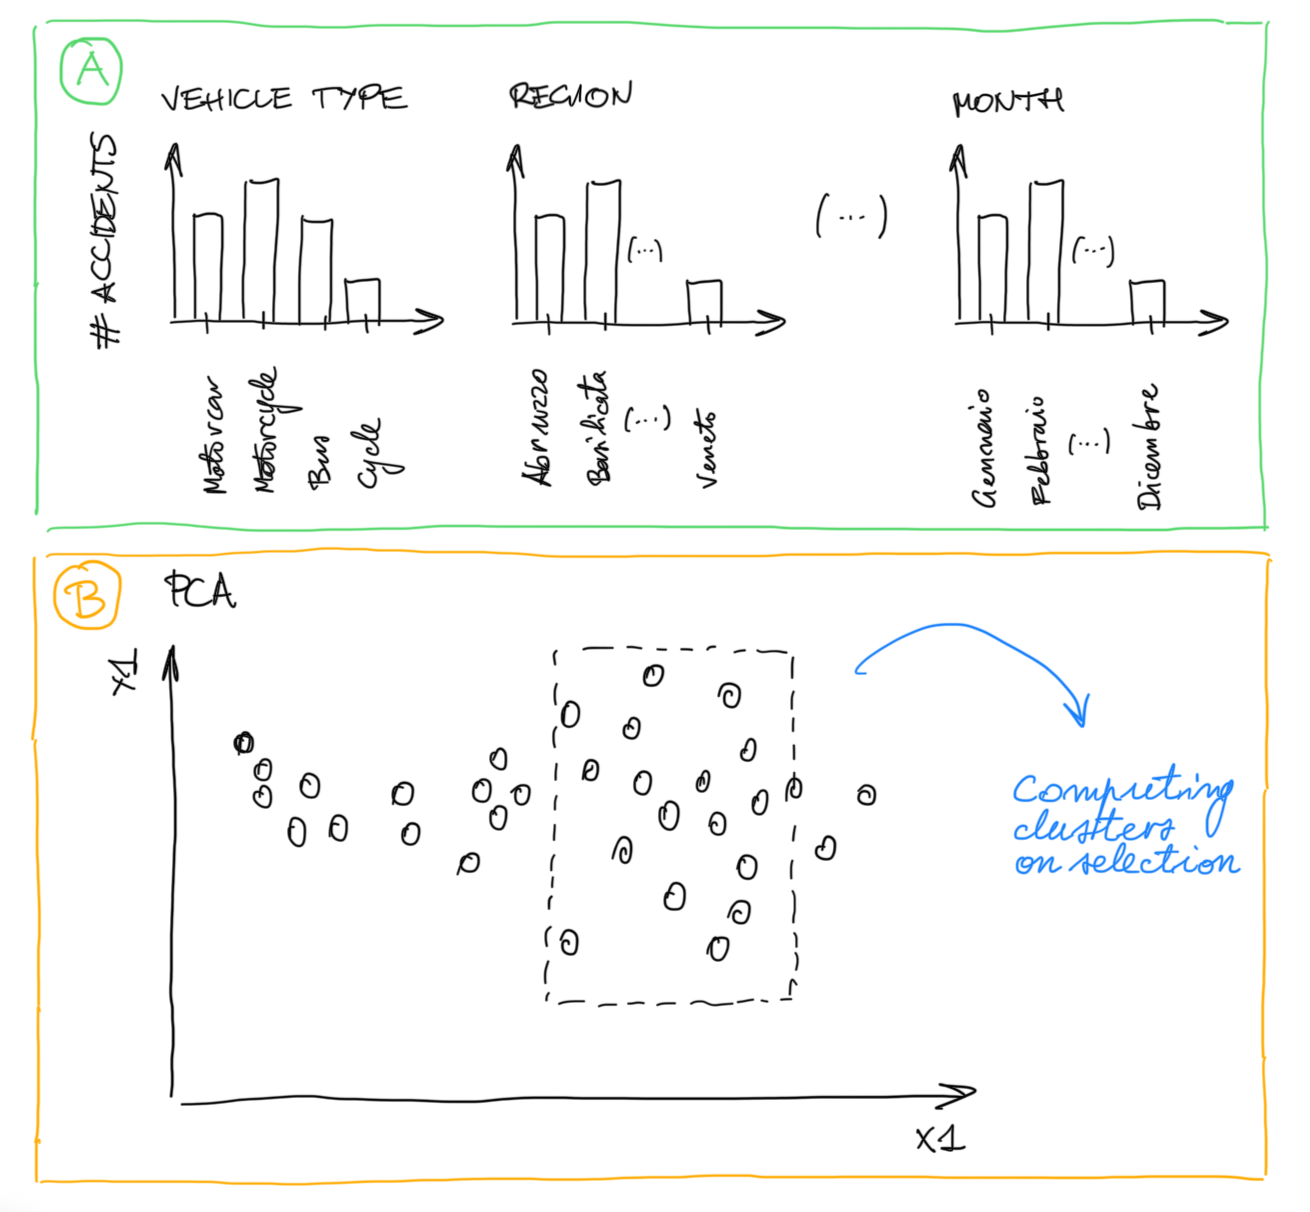
\includegraphics[width=\linewidth]{draft.png}
\caption{Draft of the visualization system}
\label{fig:draft}
\end{figure}

The system is composed of two main sections as shown in Figure \ref{fig:draft}.

In section A the number of accidents for each main attribute in the dataset
it's visualized. This is is done with a number of bar charts that use the categorical
values on the bottom axis and show the number of accidents on the vertical axis.
These charts are coordinated beetween each other. 
As an example, selecting the accidents that occurred between January and March
also highlights the road type and the kinds of vehicles involved.

In section B, the result of PCA over the dataset is presented to the user. 
Data points can be colored according to the categorical attributes of the dataset:
vehicle type, road type etc.
The PCA graph is coordinated with the graphs in section A.
As an example, selecting the accidents between January and March on section A higlights
the relative data points on the PCA graph, and vice versa.
Furthermore, the user can visually trigger an analytic by requesting the system
to find clusters (\textit{e.g. k-means}) in a selection over the PCA graph.

\section*{Dataset Details}

\begin{tabularx}{\textwidth} {| >{\bfseries}l | X |} 

\hline
Attribute name & \textbf{Description} \\
\hline\hline

Area code & ID of Region or Province \\
\hline
Area description & Name of Region or Province \\
\hline
Road type code & Number identifying a road type. Identifies motorways, urban roads and other type\\
\hline
Road type description &  Textual version of the attribute above \\
\hline
Road section code & Number identifying a road section. Identifies: tunnel, bend, crossroad, traffic circle, bump/slope or bottleneck, straight stretch, level crossing. \\
\hline
Road section description & Textual version of the attribute above \\
\hline
Accident type code &  Number identifying the accident type. Identifies:
accidents between vehicles, vehicle-pedestrian accients and accidents involving
a single vehicle. \\ 
\hline
Accident type descripiton &  Textual version of the attribute above \\
\hline
Vehicle type code &  Number identifying the vehicle involved in the
accident. Identifies: truks and motor units, cycles, tram, other vehicles, bus
or trolley-bus, mini cars, three-wheeler or motor-van, motorcars, motorcycles,
mopeds \\
\hline
Vehicle type description &  Textual version of the attribute above \\
\hline
Month number &  Month number \\
\hline
Month name &  Month name \\
\hline
Year &  Year number. Dataset contains only data for 2024 \\
\hline
Observations &  Number of accidents occurred with the specified attributes \\
\hline
\end{tabularx}

\end{document}
